% Revisado por Cristina el día 12/03/2013

\srsfuncion{Introducir plan de vuelo}
	Esta función debe añadir un nuevo vuelo a la lista de vuelos de la compañía aérea.

	\begin{enumerate}
		\item \textit{Prioridad}: alta.
		\item \textit{Entradas}
		\begin{enumerate}
			\item Los campos a introducir por el usuario son: \gls{numero_de_vuelo}, fecha y hora de origen y llegada, aeropuerto de origen y destino, el modelo de avión y el  precio total según la clase (turista, turista superior, business y primera) y tipo de pasajero (adulto, niño y bebé).
			\item El número de vuelo caracteriza e identifica unívocamente a todos los vuelos operados por la compañía. Si dicho parámetro es introducido, todos los demás deben ser ignorados en la búsqueda. Se ha de comprobar que el formato del número de vuelo se corresponde con una sucesión de 4 carácteres numéricos (si el número de caracteres es menor que 4 se completará con \verb|0| por la izquierda).
			\item Las fechas y horas introducidas deben ser válidas.
			\item Los aeropuertos de origen y destino son un conjunto finito y han de haber sido configurados previamente. Internamente se componen de nombre, ciudad y código \gls{IATA}; externamente se visualizan como una secuencia de texto configurada. El usuario podrá seleccionar uno entre ellos para cada entrada (operación que se puede abreviar introduciendo el código IATA).
			\item El modelo de avión tiene que estar disponible en las fechas indicadas, así como en un correcto estado para su funcionamiento. Dicho modelo debe estar registrado en el inventario.
		\end{enumerate}
		\item \textit{Flujo de operaciones}
		\begin{enumerate}
			\item Se muestra un formulario con los campos anteriormente descritos.
			\item El administrativo completa obligatoriamente todos los campos.
			\item El administrativo confirma la creación del nuevo plan de vuelo.
		\end{enumerate}
		\item \textit{Respuesta a situaciones no previstas}
		\begin{enumerate}
			\item Si algún campo introducido no es válido, se indica y se da la opción de introducirlo de nuevo.
			\item Si no se puede acceder a la base de datos, se muestra un mensaje de error y se da la opción de reintentar o abortar el proceso.
		\end{enumerate}
	\end{enumerate}
	
\begin{figure}[ht]\centering
	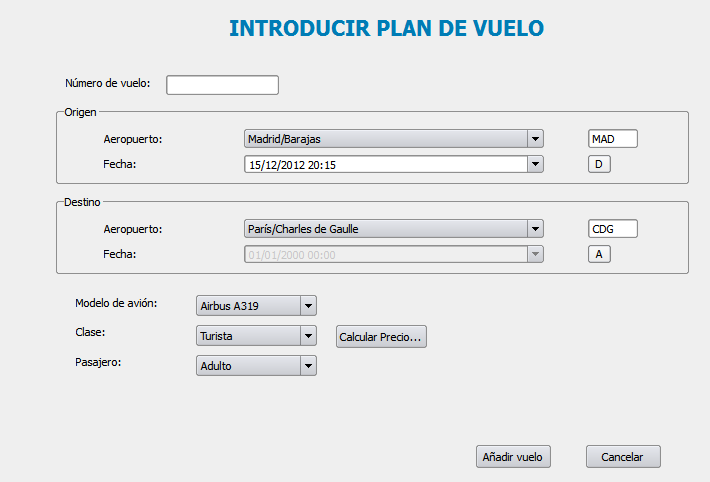
\includegraphics[scale=.6]{imagenes/introducirPlanDeVueloImagen.png}
	\caption{Pantalla aproximada de como introducir un nuevo vuelo}
\end{figure}
